\documentclass[10 pt,usenames,dvipsnames, oneside]{article}
\usepackage{../../../modelo-ensino-medio}



\begin{document}

\begin{center}
  \begin{minipage}[l]{3cm}

\includegraphics[width=2cm]{logo}    
\end{minipage}\hfill
\begin{minipage}[r]{.8\textwidth}
 {\Large \scshape Atividade: Jornada até a escola}  
\end{minipage}
\end{center}
\vspace{.2cm}

\ifdefined\prof
\begin{objetivos}
\item \textbf{LAF1} Compreender função como uma relação de dependência entre duas variáveis, as ideias de domínio, contradomínio e imagem, e suas representações algébricas e gráficas e utilizá-las para analisar, interpretar e resolver problemas em contextos diversos, inclusive fenômenos naturais, sociais e de outras áreas.
\end{objetivos}

\begin{goals}
\begin{enumerate}

\item[OE1] Representar pontos no plano cartesiano a partir de uma situação real.

\item[OE2] Estabelecer uma função a partir da seleção de pontos em um sistema cartesiano, associando a univocidade à identificação de apenas um ponto para cada valor da abscissa.

\end{enumerate}

\tcblower

\begin{itemize}
\item Durante a discussão, chame a atenção para a necessidade de certificar-se da associação de um único valor de ordenada para cada valor de abscissa.

\item Discuta com os estudantes sobre o significado dos segmentos de reta que conectam os pontos.
\end{itemize}

\end{goals}

\bigskip
\begin{center}
{\large \scshape Atividade}
\end{center}
\fi

Leonardo mora a \(6\) km da escola onde estuda e utiliza o transporte escolar, que o busca na porta de sua casa. Em um certo dia, o percurso de Leonardo até sua escola foi assim: Ele estava na porta de casa às \(7\) horas, como de costume, mas o transporte escolar atrasou, passando em sua casa somente às \(7h05min\). Leonardo entrou na van e sentou no penúltimo lugar vago. Ainda faltava Marina. “Ela mora a \(3\) km da minha casa!”, lembrou Leonardo. Às \(7h10min\) em ponto, o transporte escolar chegou à casa de Marina, que já estava pronta aguardando para embarcar. Para tentar compensar o atraso, o motorista resolveu tomar um atalho, mas a estratégia não funcionou. Às \(7h15min\) precisou ficar parado por \(5\) minutos em frente a uma cancela aguardando um trem de carga passar. Finalmente, às \(7h25min\) chegaram à escola, \(5\) minutos antes do sinal tocar.

No plano cartesiano a seguir, o eixo horizontal indica o tempo em minutos e o eixo vertical a distância percorrida em quilômetros. Os pontos marcados correspondem às distâncias percorridas por diversos estudantes da escola a cada \(5\) minutos no período das \(7h\) às \(7h30min\) da mesma manhã descrita na situação acima.

\phantomsection\label{\detokenize{AF106-4:fig-pontos-jornada}}
\begin{figure}[H]
\centering

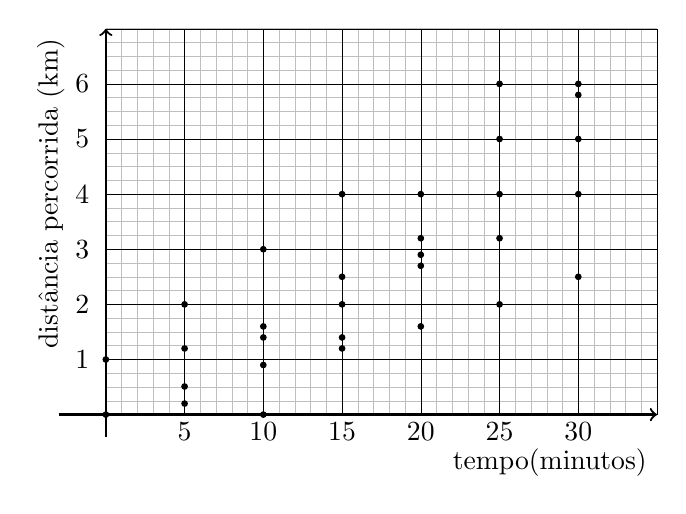
\begin{tikzpicture}
\tikzstyle{ponto}=[circle, minimum size=2pt, inner sep=0, draw=black, fill=black, shift only]
\begin{scope}[yscale=.7]
\draw[help lines,xstep=.2,ystep=.25, lightgray] (0,0) grid (7,7);
\draw[help lines, black, xstep=1, ystep=1] (0,0) grid (7,7);
\draw[thick,->](-.6,0)--(7,0) node[below left, yshift =-.3cm]{tempo(minutos)};
\draw[thick,->](0,-.4)--(0,7) node[rotate=90,left,yshift =.7cm]{ distância percorrida (km)};
\foreach \x in {5, 10, ..., 30}
\draw(.2*\x,-.3)node{\x};
\foreach \y in {1, 2, 3, 4, 5, 6}
\draw(-.3, \y)node{\y};
\node[ponto] at(0,0){};\node[ponto] at(0,1){};\node[ponto] at(1,.2){};\node[ponto] at(1,.51){};\node[ponto] at(1,1.2){};\node[ponto] at(1,2){};\node[ponto] at(2,0){};\node[ponto] at(2,0.9){};\node[ponto] at(2,1.4){};\node[ponto] at(2,1.6){};\node[ponto] at(2,3){};\node[ponto] at(3,1.2){};\node[ponto] at(3,2.5){};\node[ponto] at(3,1.4){};\node[ponto] at(3,2){};\node[ponto] at(3,4){};\node[ponto] at(4,1.6){};\node[ponto] at(4,2.7){};\node[ponto] at(4,2.9){};\node[ponto] at(4,3.2){};\node[ponto] at(4,4){};\node[ponto] at(5,2){};\node[ponto] at(5,3.2){};\node[ponto] at(5,4){};\node[ponto] at(5,5){};\node[ponto] at(5,6){};\node[ponto] at(6,2.5){};\node[ponto] at(6,4){}; \node[ponto] at(6,5){};\node[ponto] at(6,5.8){};\node[ponto] at(6,6){};
\end{scope}
\end{tikzpicture}
\end{figure}


\begin{enumerate}
\item {} 
Conecte os pontos que correspondem à jornada de Leonardo, desde a porta da sua casa até a chegada à escola, no dia descrito acima.

\item {} 
Faça uma estimativa da distância a que Leonardo estará de sua casa às \(7h07min\).

\item {} 
Escolha um conjunto de pontos que possa representar a jornada de um outro estudante da sua casa à escola e descreva essa jornada.

\end{enumerate}

\ifdefined\prof
\begin{solucao}
\begin{enumerate}

\item A jornada de Leonardo é descrita pelo gráfico abaixo:

\begin{center}
\begin{tikzpicture}

\tikzstyle{ponto}=[circle, minimum size=2pt, inner sep=0, draw=black, fill=black, shift only]
\begin{scope}[yscale=.7, every node/.style={black}, every path/.style={black}]
\draw[help lines,xstep=.2,ystep=.25, lightgray] (0,0) grid (6.5,6.2);
\draw[help lines, black, xstep=1, ystep=1] (0,0) grid (6.5,6.2);
\draw[thick,->](-.6,0)--(6.5,0) node[below left, yshift =-.2cm]{\tiny tempo(minutos)};
\draw[thick,->](0,-.4)--(0,6.2) node[rotate=90,left,yshift =.7cm]{\tiny distância percorrida (km)};
\foreach \x in {5, 10, ..., 30}
\draw(.2*\x,-.3)node{\x};
\foreach \y in {1, 2, 3, 4, 5, 6}
\draw(-.3, \y)node{\y};
\node[ponto] at(0,0){};\node[ponto] at(0,1){};\node[ponto] at(1,.2){};\node[ponto] at(1,.51){};\node[ponto] at(1,1.2){};\node[ponto] at(1,2){};\node[ponto] at(2,0){};\node[ponto] at(2,0.9){};\node[ponto] at(2,1.4){};\node[ponto] at(2,1.6){};\node[ponto] at(2,3){};\node[ponto] at(3,1.2){};\node[ponto] at(3,2.5){};\node[ponto] at(3,1.4){};\node[ponto] at(3,2){};\node[ponto] at(3,4){};\node[ponto] at(4,1.6){};\node[ponto] at(4,2.7){};\node[ponto] at(4,2.9){};\node[ponto] at(4,3.2){};\node[ponto] at(4,4){};\node[ponto] at(5,2){};\node[ponto] at(5,3.2){};\node[ponto] at(5,4){};\node[ponto] at(5,5){};\node[ponto] at(5,6){};\node[ponto] at(6,2.5){};\node[ponto] at(6,4){};\node[ponto] at(6,5){};\node[ponto] at(6,5.8){};\node[ponto] at(6,6){};
\draw[thick, session3](0,0)--(1,0)--(2,3)--(3,4)--(4,4)--(5,6)--(6,6);
\end{scope}
\end{tikzpicture}
\end{center}

\item Aproximadamente $1{,}25$ km

\item Resposta pessoal.

\end{enumerate}

\end{solucao}
\fi

\end{document}